\subsection{Thermodynamics} 

%\DTMnewdatestyle{dateupdated}{〈definition 〉

Answers to M\Alph{subsection} problems are on page \pageref{thermo_prob_answers}.  \textbf{\textcolor{red}{Updated \DTMnow.}}


%--------------------------------------------------------------------------------------------------------------
\begin{Exercise}
A tennis ball is thrown against a wall and bounces back.  
As shown in the series of drawings below, during the time it is in contact with the wall, its shape is gradually deformed as one side of it is compressed.  It returns to its original shape as it bounces back.
\begin{center}

\includegraphics[scale=0.9]{M_problems/thermo/tennis_ball_hitting_wall.pdf}
\end{center}
(a)~Draw a series of vectors showing the magnitude and direction of the force $\vv{F}$ of the wall on the tennis ball for each of the five pictures. 
(b)~Draw a rough, qualitative graph showing the magnitude of the force of the ball on the wall as a function of time during the collision.  
(c)~If the mass of the ball is 58~grams, and the ball hits the wall at a speed of 20~m/s and bounces back at the same speed, what is the change in momentum $\Delta\vv{p}$ of the tennis ball? 
(d)~Suppose that the actual collision occurs over a short time of just 2~milliseconds.  What is the average force of the ball on the wall during that time?  

[Hints: For part (d), you'll want to remember some things from physics 131.  First, what does the ``impulse-momentum theorem'' tell you about the relationship between $\Delta\vv{p}$ and $\vv{F}$? Second, what did you learn in your calculus class about how to find the average value of a function like, say, $\vv{F}(t)$?]
\end{Exercise}
\begin{Answer}
(c) 2.32 kg$\cdot$m/s (d) 1160 N
\end{Answer}


%--------------------------------------------------------------------------------------------------------------
\begin{Exercise}
In a hailstorm, 500 hailstones hit the glass windshield of your car during one 30-second interval.  The windshield has an area of 1.2~m$^2$, and is tilted at $45\degree$ from vertical.  The hailstones are falling straight down at a speed of 8~m/s, and each one has a mass of 5~grams.  Assuming that the collisions are elastic and that your car is not moving, find 
(a)~the average force and (b)~the average pressure on the windshield during this interval.
\end{Exercise}
\begin{Answer}
(a) 0.943 N (b) 0.785 Pa
\end{Answer}


%--------------------------------------------------------------------------------------------------------------
\begin{Exercise}
Suppose that $5\times10^{23}$ nitrogen (N$_2$) molecules strike a wall every second.  Assume the molecules hit the wall head-on with a speed of 300~m/s and collide elastically.  If the wall has an area of 8~cm$^2$, what is the pressure exerted on the wall? 
\end{Exercise}
\begin{Answer}
17.4 kPa
\end{Answer}


%--------------------------------------------------------------------------------------------------------------
\begin{Exercise}
How much energy is required to change a 100-gram block of ice from solid ice at $-25~\degree$C to liquid water at $60~\degree$C?  Some of the values in the table below may be helpful.

\begin{center}
\textbf{Thermodynamic Properties \\ of Water and Ice} \\
\begin{tabular}{l l}
\hline
melting point of ice & 0$~\degree$C \\
boiling point of water & 100$~\degree$C \\
density of ice & 917 kg/m$^3$ \\
density of water & 1000 kg/m$^3$ \\
latent heat of fusion $L_\text{f}$ & 334 kJ/kg \\
latent heat of vaporization $L_\text{v}$ & 2260 kJ/kg \\
specific heat of ice & 2090 J/(kg$\cdot \degree$C) \\
specific heat of liquid water & 4186 J/(kg$\cdot \degree$C)
\end{tabular}
\end{center}
\end{Exercise}
\begin{Answer}
63.7 kJ
\end{Answer}


%--------------------------------------------------------------------------------------------------------------
\begin{Exercise}
You have a cup of coffee that's too hot to drink.  Which will cool the coffee more effectively: adding a 40-gram ice cube (at $0~\degree$C) to the coffee, or adding 40 grams of liquid nitrogen (at 77~K) to the coffee?  You can assume that the nitrogen boils away, leaving as a gas at a temperature of 77~K.  (You'll need to look up some values nitrogen. But you can assume that the coffee is American coffee, which means that it's essentially the same as water.)
\end{Exercise}
\begin{Answer}
The ice cube provides more cooling.  The advantages of the liquid nitrogen are (1) that it doesn't dilute the coffee, and (2) that it makes a great spectacle with roiling mist pouring out of the cup. 
\end{Answer}


%--------------------------------------------------------------------------------------------------------------
\begin{Exercise}
The latent heat of vaporization $L_v$ of water is 2260~kJ/kg. Suppose you have a beaker of 250~ml of water already at $100~\degree$C and you wish to boil water away at a rate of one third of a gram per second by running current through a 12-ohm heater.  What current is required through the heater in order to achieve the desired rate of boiloff? 
\end{Exercise}
\begin{Answer}
About 8 amps.
\end{Answer}


%--------------------------------------------------------------------------------------------------------------
\begin{Exercise}
(a) A 5-liter vessel contains 2~moles of helium gas (monatomic) at 8~atm.  
What is the average translational kinetic energy of the helium atoms? 
(b)~Same problem as part (a), but now suppose the gas is oxygen, which is diatomic. What is the average translational kinetic energy of the oxygen molecules?
\end{Exercise}
\begin{Answer}
(a) $5.05\times10^{-21}$~J (b) still $5.05\times10^{-21}$~J 
\end{Answer}


%--------------------------------------------------------------------------------------------------------------
\begin{Exercise}
(a) A 5-liter vessel contains 2~moles of helium gas (which is monatomic) at 8~atm.  What is the total thermal energy of the gas? (That is, of all of the helium atoms.) 
(b) Same problem as part (a), but now suppose the gas is oxygen, which is diatomic. What is the total thermal energy of the gas?  
(c)  Same problem, but what if the gas is methane?\end{Exercise}
\begin{Answer}
(a) 6.06 kJ (b) 10.10 kJ (c) 12.1 kJ
\end{Answer}



%--------------------------------------------------------------------------------------------------------------
\begin{Exercise}
An ideal gas is expanded along the path shown below on the left, described by $P=\alpha V^2$, where $\alpha=5\text{~atm/m}^6$.   The gas is expanded to twice its original volume of 1~m$^3$.  How much work is done on the gas in the process?
\end{Exercise}
\begin{Answer}
$-1.18$ MJ
\end{Answer}

\hspace{\fill}
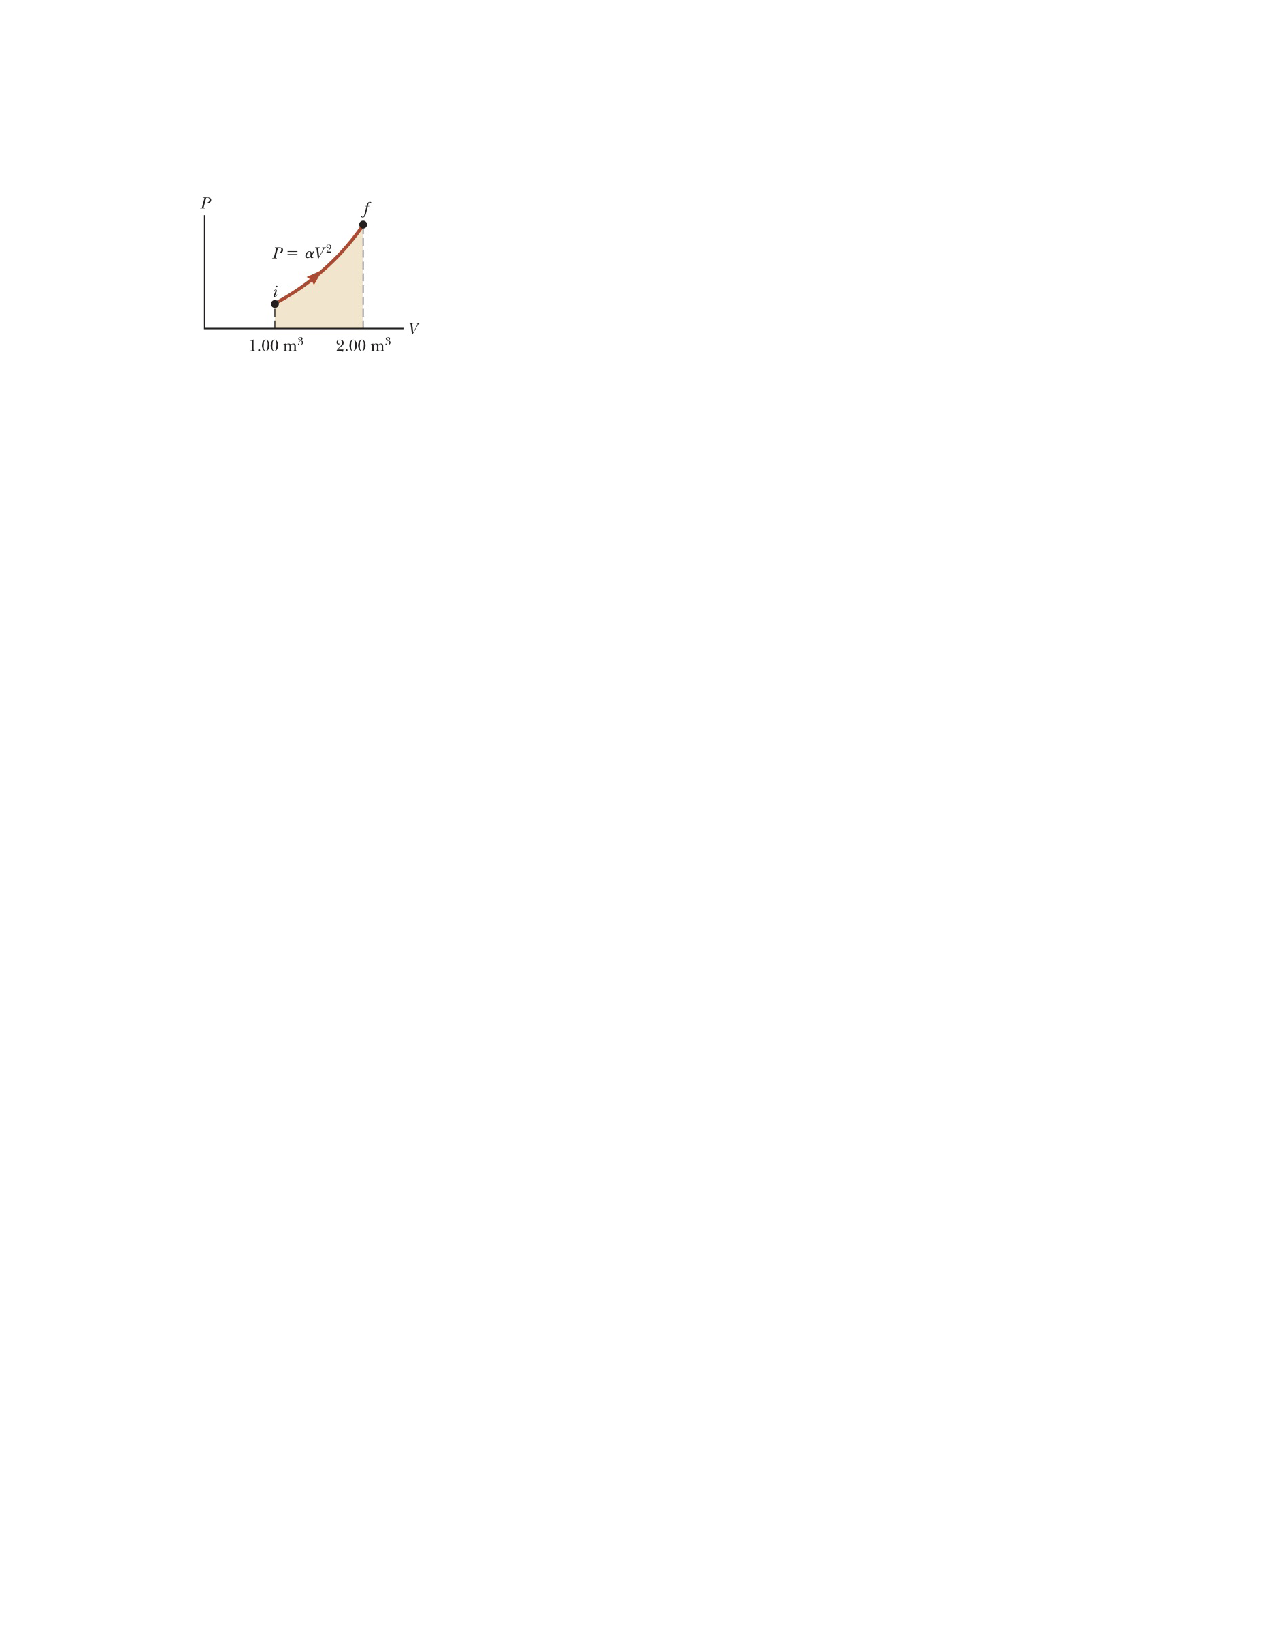
\includegraphics{M_problems/thermo/volume_squared_process.pdf}
\hspace{\fill}
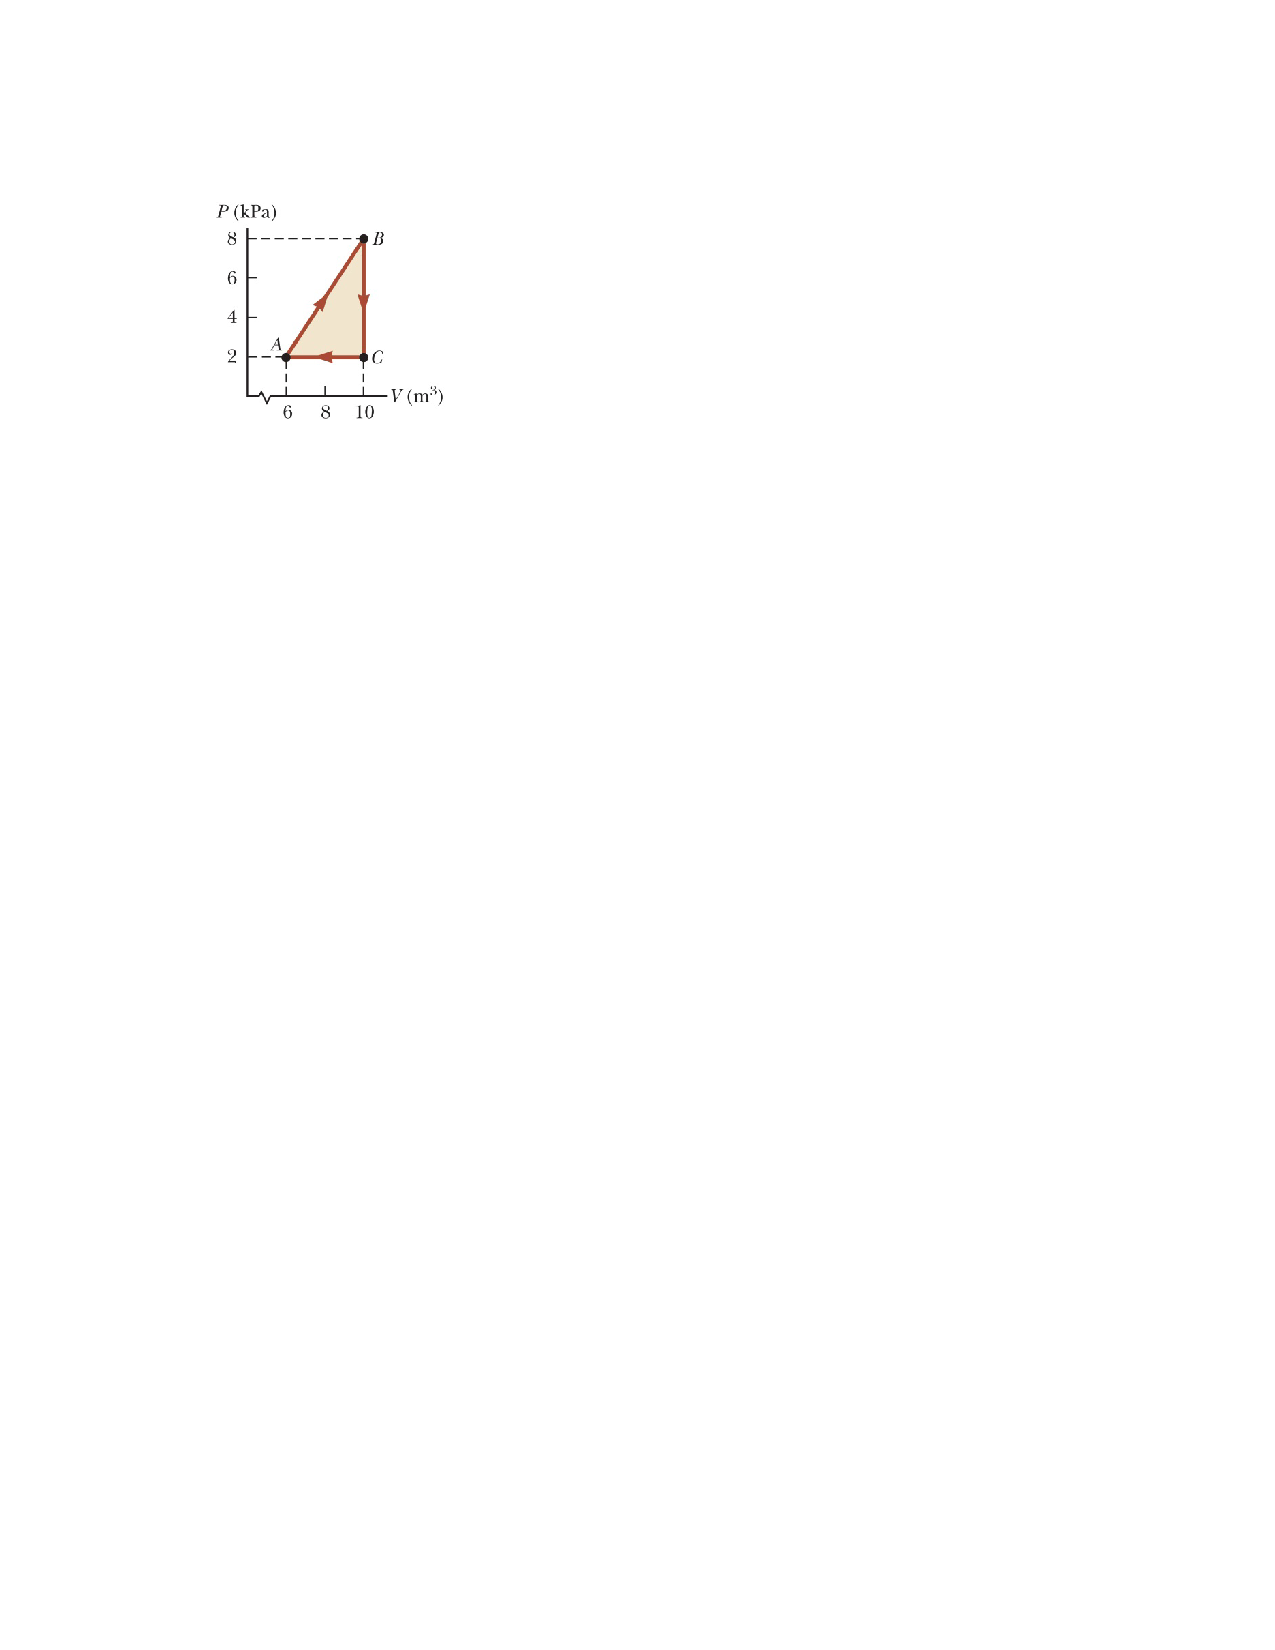
\includegraphics{M_problems/thermo/triangle_process.pdf}
\hspace{\fill}


%--------------------------------------------------------------------------------------------------------------
\begin{Exercise}
Consider an ideal gas taken through the cyclic process shown in the figure above, on the right.  
(a)~What are the signs of $W$, $Q$, and $\Delta E$ for each of the three processes AB, BC, and CA?  
(b)~Find the net energy transferred to the system by heat during one complete cycle.  
\end{Exercise}
\begin{Answer}
(a) \raisebox{-0.30in}{
\begin{tabular}{| c | c | c | c |}
\hline
& $W$ & $Q$ & $\Delta E$ \\ \hline
$AB$ & $-$ & + & + \\ \hline
$BC$ & 0 & $-$ & $-$ \\ \hline
$CA$ & + & $-$ & $-$ \\ \hline
\end{tabular} 
}

\hspace{0.55in}(b) $Q_\text{net}= 12$~kJ
\end{Answer}



%--------------------------------------------------------------------------------------------------------------
\begin{Exercise}
A 2-mole sample of helium gas initial at 300~K and 0.4~atm of pressure is compressed isothermally to 1.2~atm.  Find (a)~the final volume of the gas, (b)~the work done on the gas, and (c)~the energy transferred by heat.
\end{Exercise}
\begin{Answer}
(a) 0.041 m$^3$ (b) $+5.48$ kJ (c) $-5.48$ kJ.
\end{Answer}


\figuretoright{0.3}{M_problems/thermo/isothermal_and_adiabatic_processes.pdf}{
%--------------------------------------------------------------------------------------------------------------
\begin{Exercise}
In the two processes shown to the right, one of the processes shown is isothermal, and the other is adiabatic.  
(a) Which is which?  
(b) Each process is performed on 0.1~moles of nitrogen gas, starting at $P=3$~atm and $V=1$~liter.  
Both processes have a final volume of $V=3$~liters.  
How much heat energy $Q$ is expelled by the gas in each case?
\end{Exercise}
\begin{Answer}
(b) One of the two expels 330 joules.
\end{Answer}
}

%--------------------------------------------------------------------------------------------------------------
\begin{Exercise}
A 4-liter vessel of a diatomic ideal gas is carried through a closed cycle.  The gas is initially at 1 atm and 300 K.  First, the pressure is tripled at constant volume.  Then the gas expands adiabatically back to 1 atm.  Finally, the gas is compressed isobarically to its original volume.  (a) Draw a PV diagram of the cycle.  (b) Find the volume of the gas at the end of the adiabatic expansion. (c) Find the temperature of the gas at the start of the adiabatic expansion.  (d)  Find the temperature at the end of the cycle.  (e) What is the net work done on the gas during the cycle?
\end{Exercise}
\begin{Answer}
(b) 8.77 liters (c) 900 K (d) 300 K (e) $-336$ J
\end{Answer}


%--------------------------------------------------------------------------------------------------------------
\begin{Exercise}
2500 joules of heat flow from a hot reservoir at 725~K to a cold reservoir at 310~K when the two reservoirs are briefly brought into direct contact with each other.  Calculate the change in entropy of (a)~the hot reservoir, (b)~the cold reservoir, and 
(c)~the Universe (that is, $\Delta S_\text{net}$).
\end{Exercise}
\begin{Answer}
(a) $-3.45$ J/K (b) $+8.06$ J/K (c) $+4.61$ J/K
\end{Answer}


%--------------------------------------------------------------------------------------------------------------
\begin{Exercise}
You and your roommates need a new refrigerator.  At the ``E-Z appliances'' store, a salesman in a cheap suit with slicked-back hair shows you the ``Wonder DreamFridge 2000 Plus''.  According to the sticker on it, the DreamFridge uses a mere 100~W of power to remove 100~kJ of heat per minute from the $2~\degree$C interior of the Fridge.  (The fine print reveals this is true if the ambient temperature in the kitchen is $22~\degree$C.)  Should you buy it? Or is this one of those offers that's too good to be true---which is to say, false? 
\end{Exercise}
\begin{Answer}
The offer is indeed too good to be true.  But you still need to explain how you know that the details on the DreamFridge tag must be false, besides the obviously unprepossessing store name and the sleazy salesman.
\end{Answer}





\vspace{0.7in}

\textbf{Answers to Selected {\thesubsection} Problems:}
\label{thermo_prob_answers}
%\shipoutExercise
\shipoutAnswer

\cleardoublepage
